\section{Network Layer (IP \& Routing)}

\subsection{Introduction to IP addressing}
\begin{itemize}
	\item IPv4 address = 32 bits (a.b.c.d), identifies interface (host/router can have multiple interfaces).
	\item Subnet vs host split via CIDR: a.b.c.d/$x$ where $x$ = prefix length (subnet mask).
	\item Example: 192.168.1.178/24 $\Rightarrow$ subnet 192.168.1, host 178.
	\item Hierarchical addressing enables routing scalability; ISPs advertise prefixes.
	\item Forwarding uses \textbf{longest prefix match}.
	\item \textbf{Address discovery protocols:}
\end{itemize}

\begin{center}
    \textbf{IP Packet Diagram}
    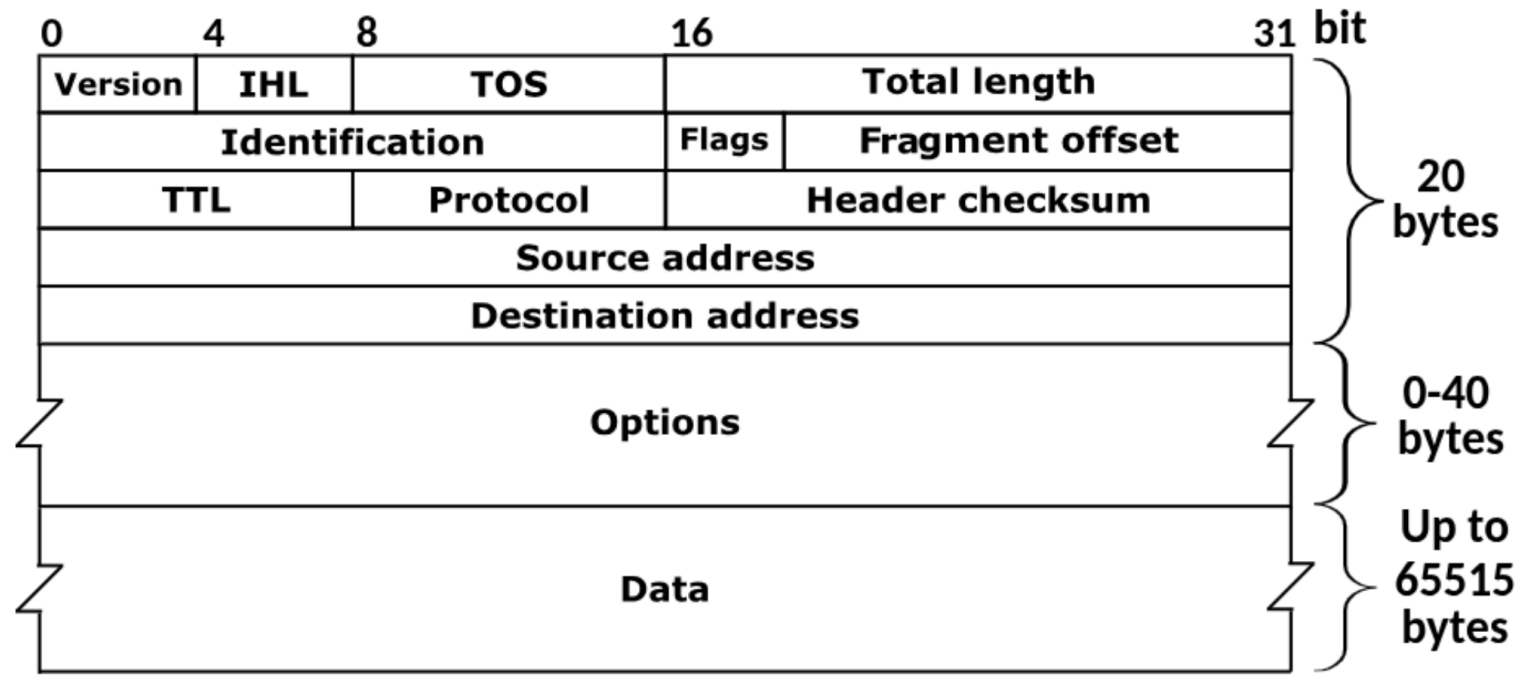
\includegraphics[width=0.9\columnwidth]{images/ip_packet_diagram.png}
\end{center}
